\documentclass[14pt,]{article}
\usepackage{lmodern}
\usepackage{amssymb,amsmath}
\usepackage{ifxetex,ifluatex}
\usepackage{fixltx2e} % provides \textsubscript
\ifnum 0\ifxetex 1\fi\ifluatex 1\fi=0 % if pdftex
  \usepackage[T1]{fontenc}
  \usepackage[utf8]{inputenc}
\else % if luatex or xelatex
  \ifxetex
    \usepackage{mathspec}
  \else
    \usepackage{fontspec}
  \fi
  \defaultfontfeatures{Ligatures=TeX,Scale=MatchLowercase}
\fi
% use upquote if available, for straight quotes in verbatim environments
\IfFileExists{upquote.sty}{\usepackage{upquote}}{}
% use microtype if available
\IfFileExists{microtype.sty}{%
\usepackage{microtype}
\UseMicrotypeSet[protrusion]{basicmath} % disable protrusion for tt fonts
}{}
\usepackage[margin=0.1in]{geometry}
\usepackage{hyperref}
\hypersetup{unicode=true,
            pdftitle={NZ SRW Modelling Report},
            pdfauthor={Anthony Davidson},
            pdfborder={0 0 0},
            breaklinks=true}
\urlstyle{same}  % don't use monospace font for urls
\usepackage{longtable,booktabs}
\usepackage{graphicx,grffile}
\makeatletter
\def\maxwidth{\ifdim\Gin@nat@width>\linewidth\linewidth\else\Gin@nat@width\fi}
\def\maxheight{\ifdim\Gin@nat@height>\textheight\textheight\else\Gin@nat@height\fi}
\makeatother
% Scale images if necessary, so that they will not overflow the page
% margins by default, and it is still possible to overwrite the defaults
% using explicit options in \includegraphics[width, height, ...]{}
\setkeys{Gin}{width=\maxwidth,height=\maxheight,keepaspectratio}
\IfFileExists{parskip.sty}{%
\usepackage{parskip}
}{% else
\setlength{\parindent}{0pt}
\setlength{\parskip}{6pt plus 2pt minus 1pt}
}
\setlength{\emergencystretch}{3em}  % prevent overfull lines
\providecommand{\tightlist}{%
  \setlength{\itemsep}{0pt}\setlength{\parskip}{0pt}}
\setcounter{secnumdepth}{0}
% Redefines (sub)paragraphs to behave more like sections
\ifx\paragraph\undefined\else
\let\oldparagraph\paragraph
\renewcommand{\paragraph}[1]{\oldparagraph{#1}\mbox{}}
\fi
\ifx\subparagraph\undefined\else
\let\oldsubparagraph\subparagraph
\renewcommand{\subparagraph}[1]{\oldsubparagraph{#1}\mbox{}}
\fi

%%% Use protect on footnotes to avoid problems with footnotes in titles
\let\rmarkdownfootnote\footnote%
\def\footnote{\protect\rmarkdownfootnote}

%%% Change title format to be more compact
\usepackage{titling}

% Create subtitle command for use in maketitle
\providecommand{\subtitle}[1]{
  \posttitle{
    \begin{center}\large#1\end{center}
    }
}

\setlength{\droptitle}{-2em}

  \title{NZ SRW Modelling Report}
    \pretitle{\vspace{\droptitle}\centering\huge}
  \posttitle{\par}
    \author{Anthony Davidson}
    \preauthor{\centering\large\emph}
  \postauthor{\par}
      \predate{\centering\large\emph}
  \postdate{\par}
    \date{02 November, 2019}


\begin{document}
\maketitle

\#Raw data

The data is then converted into intervals for each of the years 2010,
2011, 2012 and 2013.

A table of the raw results as the year increase

\begin{longtable}[]{@{}rrrrrr@{}}
\toprule
year & n & mY & low.qt & high.qt & sd\tabularnewline
\midrule
\endhead
2010 & 3 & 2.666667 & 1.605851 & 3.727482 & 0.5773503\tabularnewline
2011 & 15 & 2.866667 & 2.673022 & 3.060312 & 0.3518658\tabularnewline
2012 & 25 & 3.240000 & 2.919170 & 3.560830 & 0.7788881\tabularnewline
2013 & 45 & 3.311111 & 3.056488 & 3.565734 & 0.8480518\tabularnewline
\bottomrule
\end{longtable}

\#\#Raw data plots The raw intervals can be presented as different means
and confidence intervals as the length of the study increases:

We can also plot these as bar charts that show this more obviously:

What is interesting is that in 2011 there were more intervals that
subsequently reduced the standard error of the estimate and the
precision increased.

\textbf{My idea of why this has happened is as follows:}

At the time of collection in 2011 the number of possible intervals
greater than 5 was very unlikely (as there where only 5 years of
research). This meant that the overall error of the estimate was reduced
as there was very few ``chances'' of obtaining a calving interval of 5
or 6 even though there may have been quite a few. The following
estimates then picked these up and the error in the estimate increased
again.

The upgrade for publication standard: \textbf{working in the R
enviroment}

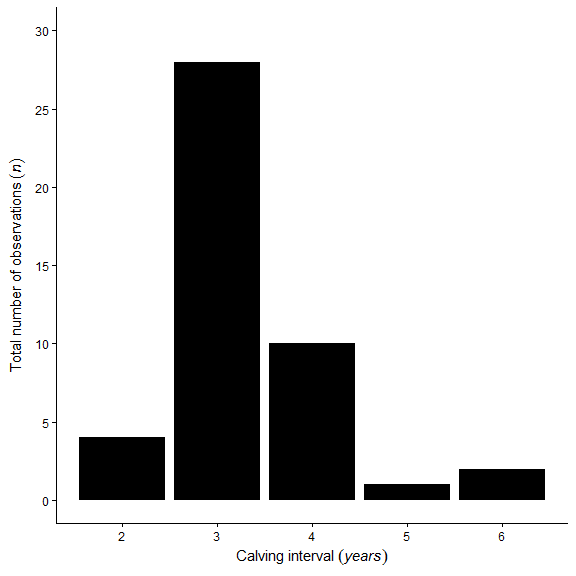
\includegraphics{ESA-SRW-modelling-paper_files/figure-latex/raw graph 3-1.pdf}

\#Missing intervals (Bradford et al.~2008)

This is a way to see what the calving interval might be if we had in
fact missed calving events that happened before or after the study
period.

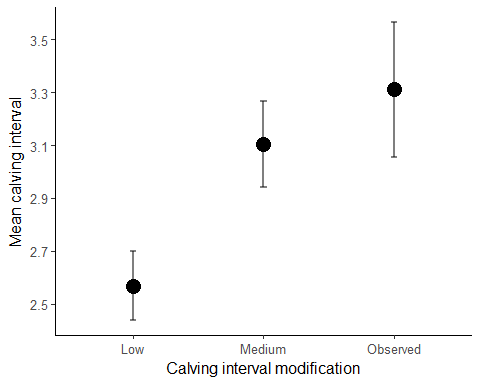
\includegraphics{ESA-SRW-modelling-paper_files/figure-latex/missing intervals plot3-1.pdf}

The error gets smaller as the variance in the estimate decreases. We are
artificially doing this here by modifying data to match what is more
biologically possible.

\begin{longtable}[]{@{}lrrrrr@{}}
\toprule
interval & n & mY & low.qt & high.qt & sd\tabularnewline
\midrule
\endhead
Low & 58 & 2.568966 & 2.437666 & 2.700265 & 0.4995461\tabularnewline
Medium & 48 & 3.104167 & 2.943089 & 3.265244 & 0.5550382\tabularnewline
Observed & 45 & 3.311111 & 3.056488 & 3.565734 &
0.8480518\tabularnewline
\bottomrule
\end{longtable}

\#Bootstrapping

\textbf{Table of parameters:} This is taken directly from my Master's
thesis. There may be updated estimates that need to be checked here.

\begin{longtable}[]{@{}rrrrrll@{}}
\toprule
n & interval & low.qt & high.qt & se.pub & author &
location\tabularnewline
\midrule
\endhead
NA & 3.12 & 3.07 & 3.17 & NA & Best et al.~2001 & South
Africa\tabularnewline
1504 & 3.15 & 3.11 & 3.18 & NA & Best et al.~2005 & South Africa
(1971-2003 Updated)\tabularnewline
NA & 3.16 & 3.13 & 3.19 & NA & Brandao et al 2010 & South Africa (
1971-2006 Updated)\tabularnewline
NA & 3.35 & NA & NA & 0.05 & Cooke et al.~2001 &
Argentina\tabularnewline
749 & 3.42 & NA & NA & 0.11 & Cooke et al.~2003 &
Argentina\tabularnewline
NA & 3.63 & NA & NA & 0.13 & Burnell 2001 & Australia\tabularnewline
\bottomrule
\end{longtable}

Bootstrap mean calving interval 1000 times and save the mean for each
bootstrap sample. Here I investigate the effect of a sample size of
10,100,1000,2000 from the observed NZ calving interval.

\#\#\#Publication plot 1000 replicates
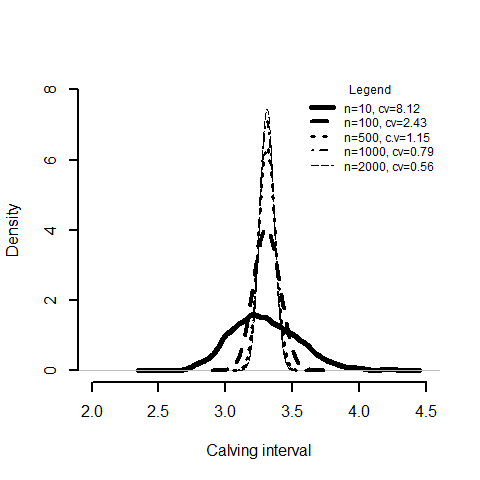
\includegraphics{ESA-SRW-modelling-paper_files/figure-latex/bootstrap plot2-1.pdf}


\end{document}
